% !TeX spellcheck = de_DE 
\chapter{Implementierung}
In meiner Abschlussarbeit präsentiere ich die praktische Lösung für das PSE-Labor der Beuth Hochschule für Technik Berlin. Die gesamte Aufgabe lässt sich in drei Bestandteile unterteilen: Register-Client, Server und Display-Client. Erstens wird Register-Client implementiert, damit wird RFID Leser am Raspberry Pi Mikrocomputer angeschlossen, alle Treiber installiert und auf Python Programmierung Sprache die Software geschrieben, die die ständige Überwachung des empfangenden von RFID Leser Daten zulässt und die Verbindung mit dem Server zulässt. Falls die empfangene Daten korrekt sind, d.h.  eine richtige MIFARE Studentenkarte oder einen richtigen RFID-Transponder abgelesen wurde, schickt die Software die abgelesene Daten zum Server ab. Der Server ist der zweite Bestandteil der Abschlussarbeit und wird mit Hilfe Django Framework, Django Finite State Machine auf Python Programming Sprache implementiert. Server enthält die Datenbank mit die Datensätzen über die alle im PSE-Labor vorhandenen ausleihenden Boards, die zum Modul im laufenden Semester registrierten Studenten und  geschehenen Ausleihe/Rückgabe-Vorgänge. Es wird von Server überprüft, ob eine von Register-Client abgelesene Studentenkarte einem zugelassenen für die Ausleihe Student gehört und die entsprechenden Information auf Display-Client geschickt. Es wird auch von Server bestätigt, ob für die Ausleihe/Rückgabe neben dem RFID-Leser gehaltenen Raspi Board dem Student ausgeliehen/vom Student zurückgegeben werden darf. Darauf aufbauend, wird der dritte Teil namens ein Display-Client als dynamische HTML-Seite realisiert, die eine Verbindung zum Server Mithilfe des HTTP-Protokolls und eingebauten im Browser Kommunikationsmittel die asynchrone Nachrichten zu schicken, bereitstellt. Für die dynamische Aktualisierung des Inhalts der Webseite und einen Zugang zum asynchronen HTTP-Client wird jQuery benutzt.
\section{Register-Client}
\label{sec:register_client}
Das folgende Kapitel beschäftigt sich mit der Implementierung des Register-Client auf Raspberry Pi Board mit angeschlossenen RFID-Leser. Dieser Teil der verteilte System lässt sich wie folgendes unterteilen. Zuerst wurde das Betriebssystem Raspbian auf Board zum Leben gebracht und dann die alle notwendigen für RFID-Leser Treiber installiert. Nach dem der RFID-Leser funktionieren angefangen und die Daten von RFID-Transponder abgelesen hat, wurde die nächste Herausforderungen gelöst: die Struktur die zu empfangenen Daten wurde verstanden, richtig bearbeitet, eine JSON-Datei erstellt und durch die HTTP-Protokoll dem Server geliefert. 

\subsection{Installation des Betriebssystem}
\label{sec:register_client:raspbian}
Der vorhandene für die Abschlussarbeit Raspberry Pi 3 Model B+ wurde nicht als Starter Kit mir übergeben, dann wurde es zusätzlich benötigt\cite[pp. 21-22]{gareth:raspi}: 
\begin{itemize}
	\item \textbf{USB-Netzteil} mit einer Nennleistung von 2,5 A (2,5 A) oder 12,5 Watt (12,5 W) und einem Micro-USB-Anschluss. 
	\item \textbf{microSD-Karte}, die als permanenter Speicher des Raspberry Pi dient; Alle von Benutzer erstellten Dateien und die installierte Software sowie das Betriebssystem selbst werden auf der microSD-Karte gespeichert.
	\item \textbf{USB-Tastatur und -Maus}, mit denen den Raspberry Pi gesteuert werden kann. Fast jede kabelgebundene oder kabellose Tastatur und Maus mit USB-Anschluss funktioniert mit dem Raspberry Pi.
	\item \textbf{Das HDMI-Kabel}, das Ton und Bilder vom Raspberry Pi auf Fernseher oder Monitor überträgt. Sie müssen nicht viel Geld für ein HDMI-Kabel ausgeben. 
\end{itemize}

Die Arbeit mit einem RaspberryPi setzt ein paar Anfangsinvestitionen voraus, die auch von den angestrebten Aufgaben und Projekten abhängen. Zuerst gäbe es die Möglichkeiten, dass der gekaufte Raspberry Pi Board bereits ein Betriebssystem darauf installiert hätte. Aber es war nicht der Fall von vorhandenen im PSE-Labor Board. Um ein Betriebssystem auf diesen Raspberry Pi zu bringen, muss eine SD-Karte mit einem Betriebssystem-Image "geflasht" werden. Dafür zunächst wurde die Distribution von der Website Raspbian.org herunterladen und die MicroSD-Karte in den Kartenleser eines vorhandenen im PSE-Labor PC eingelegt. Anschließend wurde mit dem Macintosh Disk Utility-Dienstprogramm das heruntergeladene und entpackte Betriebssystem für den RaspberryPi auf eine Speicherkarte geschrieben. Dann ist die Karte in Raspberry Pi einzulegen. Der Raspi ist damit betriebsbereit und muss für die zukünftigen Anwendungen noch konfiguriert werden. Wenn der Pi zum ersten Mal eingeschaltet wird, wird viel Text auf dem Bildschirm angezeigt. Diese werden als Startmeldungen bezeichnet. Wenn Raspbian zum ersten Mal gestartet wurde, kann es ein oder zwei Minuten dauern, um die Nutzung des freien Speicherplatzes auf der microSD-Karte optimal anzupassen. Beim nächsten Start geht es schneller. Schließlich ist kurz ein Fenster mit dem Raspberry Pi-Logo zu sehen, dann wird Terminal Fenster angezeigt, in dem es einloggt werden muss. Zum ersten Einloggen wird den Standardbenutzername "pi" und das Standardkennwort  "raspberry" verwendet. Um Register-Client vor sowohl Online-Bedrohungen als auch von Missbrauch im Labor zu schützen, wurde das Standardkennwort sofort geändert. Der nächste Schritt ist Raspbian bis zur Version "Raspbian mit dem Raspberry Pi Desktop" zu aktualisieren, damit die grafische Benutzeroberfläche und Chromium Browser zu Verfügung stehen können. Dies kann mit dem Terminalbefehl gemacht werden:
\begin{lstlisting}
sudo apt-get install lxde-core xserver-xorg xinit
\end{lstlisting}
Dann ist der Raspberry Pi erneut zu laden. Nachdem Raspberry Pi-Logo wieder angezeigt wurde, wäre der Raspbian-Desktop zu sehen. Somit gilt Betriebssystem als vollständig installiert und kann benutzt werden. Das war aber nicht der Fall mit dem vorhandenen Hardware, da es plötzlich eine Boot-Schleife vorkam, nachdem der Mikrocomputer eingeschaltet wurde und der Startvorgang nicht abgeschlossen werden konnte. Anstatt das zum Benutzung bereiteten Betriebssystem mit der grafische Benutzeroberfläche zu sehen,  wird eine Schleife erzeugt, in der die Startvorgang kontinuierlich und wiederholt ausgeführt wurde und somit eine Nutzung der Mikrocomputers unmöglich ist. Nach den mehreren Recherchen wurde es vermutet, dass es durch eine unzureichende Stromversorgung verursacht werden könnte. Es wurde aber zuerst nicht versucht, einen USB-Netzteil zu wechseln, da die anderen USB-Netzteil man durch PSE-Labor bestellen und eine Zeit abwarten muss. Jedoch wurde eine erzeugte Boot-Schleife mit einem anderen Terminalbefehl erfolgreich gelöst:
\begin{lstlisting}
sudo apt-get install --reinstall pcmanfm
\end{lstlisting}
Bei der Arbeit mit dem Mikrocomputer tritt jedoch später ein Problem mit der Stromversorgung auf. Der Fall kann im entsprechenden Kapitel \ref{sec:register_client:voltage_issue} nachgelesen werden.


\subsection{Installation der Treibers für RFID-Leser}
\label{sec:register_client:install_rfid}
Obwohl Raspbian mit einer Reihe von Software vorinstalliert ist, wird es aber zusätzlich benötigt, die Treiber für RFID-Leser zu installieren. Es sollte an dieser Stelle auch noch angemerkt werden, dass am Anfang der Entwicklungsprozess ein anderen RFID-Leser angeschlossen wurde als der, den in der Abschlussarbeit zu beschreiben und zu beobachten ist. Zuerst wurde die Treiber für Reiner SCT CyberJack RFID Basis\cite{website:4} installiert. Die Schritte sollten in der Abschlussarbeit nicht unerwähnt bleiben, da die damals für den ersten RFID-Leser installierte Treiber und Daemons (Appendix \ref{sec:appendix:daemon}) wurden endlich für den zweiten RFID-Leser benutzt, mit dem die Entwicklung der Aufgabe abgeschlossen wurde. Der Grund für die Hardwareaustausch ist die festgestellte Tatsache, dass Reiner SCT CyberJack RFID Leser die Studentenkarten nicht ablesen konnte. Obwohl in der Spezifikation es steht, dass die Reiner RFID-Leser kontaktlose RFID Chipkarten wie eID mit dem neuen Personalausweis (nPA), GeldKarte oder eTicketing unterstützt, wurde es unmöglich mit den MIFARE-Transponder 13,561 MHz Funkbereich ins Spiel zu bringen. Die Studierenden-Ausweise der Beuth sollten mit dieser Technologie gelesen werden und somit ist diese Anforderung für die vorliegende Abschlussarbeit wichtig. 

Um RFID-Leser anzuschließen, muss man den Leser über USB mit einem Raspberry Pi verbunden. Der Typ des RFID-Lesegeräts, der für die vorliegende Abschlussarbeit verwendet wird, ist ein ACR122U-A9 von Advanced Card Systems\cite{website:7}, den auf der Abbildung\ref{fig:rfid_hard} zu sehen. Zuerst müssen wir die Paketlisten aktualisieren und einige erforderliche Pakete herunterladen und installieren:\cite{website:6}
\begin{lstlisting}
sudo apt-get update
sudo apt-get install pcscd pcsc-tools pcsc-lite
sudo apt-get install libpcsclite-dev libtool
sudo apt-get install libusb-1.0-0-dev
\end{lstlisting}

\begin{wrapfigure}{l}{0.45\textwidth}
	\fbox{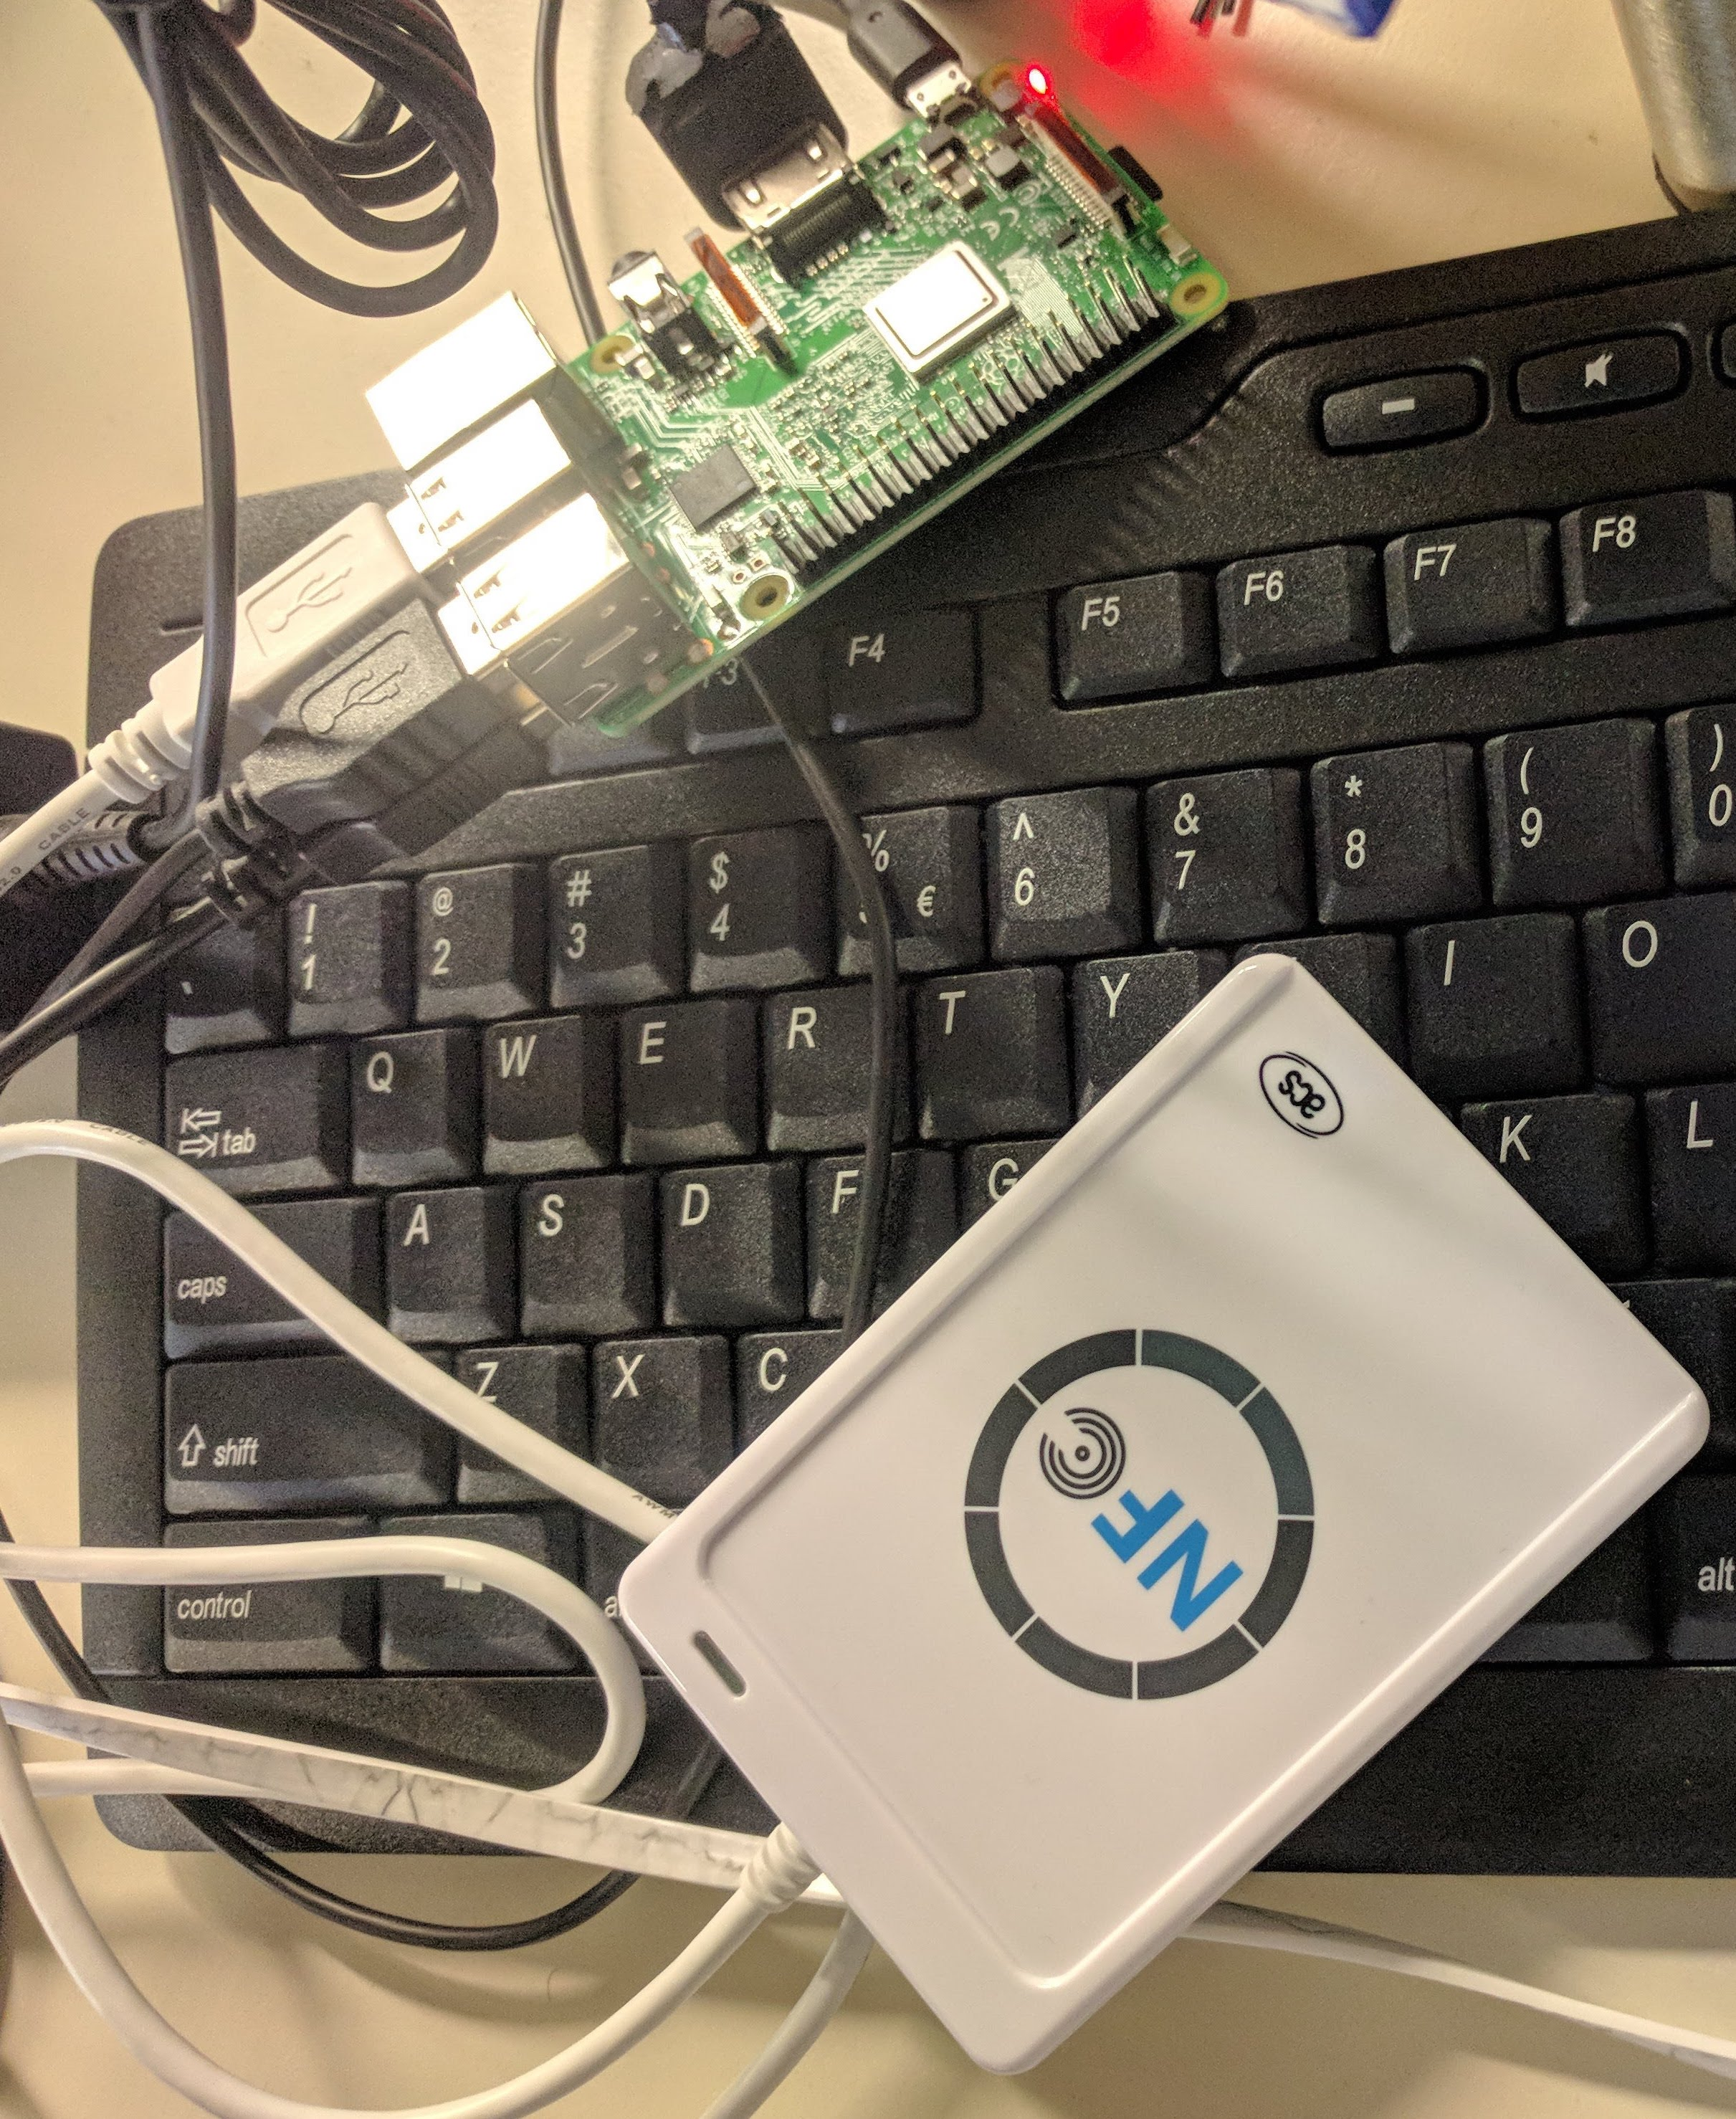
\includegraphics[width=0.42\textwidth]{gfx/rfid_hard.jpg}}
	\caption{ACR122U-A9 von Advanced Card Systems und Raspbery Pi}
	\label{fig:rfid_hard}
\end{wrapfigure}
PC/SC ist ein Standard für die Schnittstelle von Computern mit Smartcards, der auf den meisten Betriebssystemen, einschließlich Windows und Linux, verfügbar ist. PC/SC-Kopplungsgeräte benötigen einen Treiber, mit dem Anwendungen die Karte einfach erreichen können. Da PC/SC für Smartcards entwickelt wurde - und in einer Zeit, in der Smartcards nur Kontaktkarten waren funktioniert es auch mit den kontaktlosen Karten, falls RFID-Leser es unterstützt. Das Daemon-Programm für pcsc-lite namens pcscd koordiniert die Kommunikation mit Smartcard-Lesegeräten und Smartcards sowie kryptografischen Tokens, die mit dem System verbunden sind. Normalerweise wird pcscd beim Booten von /etc/init.d/pcscd gestartet. Damit können Anwendungen auf Smartcards und Lesegeräte zugreifen, ohne die Details der Karte oder des Lesegeräts zu kennen. Das Laden von Treibern für Kartenleser wird von pcscd koordiniert. Der Zweck von pcsc-lite besteht darin, eine kompatible API (Winscard) für die Migration von Windows-basierten PC / SC-Anwendungen auf Unix bereitzustellen\cite{website:5}. Die allgemeinen Zugriff auf USB-Geräte bietet eine C-Bibliothek namens libusb.  Sie soll von Entwicklern verwendet werden, um die Produktion von Anwendungen zu erleichtern, die mit USB-Hardware kommunizieren. Es ist portabel, da mit einer einzigen plattformübergreifenden API auf USB-Geräte unter Linux, MacOS, Windows usw. zugegriffen werden kann. Sie wird im Benutzermodus ausgeführt und somit für die Kommunikation der Anwendung mit einem Gerät keine besonderen Berechtigungen oder Erhöhungen erforderlich sind.\cite{website:8}

Dann laden wir die Open-Source-Bibliothek libnfc für Near Field Communication (NFC) herunter, extrahieren, konfigurieren und installieren es. Nach der erfolgreichen Installation kann den verbindenden über USB RFID-Leser mithilfe des Tools lsusb angesehen werden: es wird VendorId und ProductID angezeigt. Es ist auch notwendig die abgelesene VendorId und ProductID in der entsprechenden XML-Datei. Die Datei auf der MicroSD-Karte ist zu finden :
\begin{lstlisting}
/usr/lib/pcsc/drivers/ifd-ccid.bundle/Contents/info.plist
\end{lstlisting}

\subsection{Spannungsproblem und Lösung}
\label{sec:register_client:voltage_issue}
Nachdem der RFID-Leser angeschlossen wurde, tritt es ein weiteres Problem, das die freie Benutzung der Raspberry Pi unmöglich macht. Es wird unabhängig von der Zeit und vorherigen Geschehen eine Fehlermeldung "under voltage detected (0x000050000000)". Es wird zuerst versucht die kabellose USB-Tastatur und -Maus abzuschalten. USB eine aktive Abfrage seine Ports (Polling) benötigt, was bedeutet, dass die Anzahl der für andere Aufgaben verfügbaren CPU Zyklen geringer ist. Dies kann dazu führen, dass die CPU-Frequenz ansteigt, wodurch der Stromverbrauch höher wäre. Es wurde festgestellt, dass mit unverbundenen USB-Tastatur und -Maus die Fehlermeldung trotzt vorkommt. Nur wenn der RFID-Leser angeschaltet wurde, kam es keine neue Fehlermeldung. Dann es wurde geprüft, ob ausgewählten RFID-Leser mit dem vorhandenen Mikrocomputer überhaupt kompatibel ist und nach der Lösung gesucht, mit der die zukünftige Entwicklung weiterlaufen kann.    

Anfänglich wurde als Spannungsversorgungsteil ein USB-Netzteil von einem modernem bei Autorin der Abschlussarbeit vorhandenen zu Hause Smartphone benutzt. Das offizielle Raspberry Pi-Netzteil ist die empfohlene in der Dokumentation Wahl, jedoch wurde zuerst mit dem Mikrocomputer nicht gekauft. Ein leistungsfähiger USB-Netzteil könnte den schnell wechselnden Strombedarf des Raspberry Pi bewältigen. Nach der Besprechung des Problems mit den PSE-Labor Mitarbeiter wurde ein Samsung USB-Netzteil gegen einen Anker USB-Netzteil ausgetauscht und festgestellt, dass das Spannungsproblem mit den verbundenen sowohl USB-Tastatur und -Maus als auch RFID-Leser während des Ablesevorgangs nicht wieder erscheint. 

\subsection{Python Programmierung des RFID-Lesers}
\label{sec:register_client:smart}
Nachdem es gelingt mir, die Hardware angefahren und die ersten Studentenkarte so abzulesen, dass es ein Schallton von RFID-Leser erzeugt wurde, sollte eine weitere Aufgabe gelöst werden: die Daten von RFID-Tag auf einem auszuleihenden Raspi Board von Studentenkarte unterscheiden zu können. Es sollte ausgeschlossen werden, dass ein Ausleihe-/Rückgabevorgang angefangen wird, falls eine falsche Studentenkarte (z.B. mit einer BVG Jahresfahrkarte) am RFID-Leser präsentiert wird. Als es im Kapitel \ref{sec:theorie:mifare} erklärt wurde, sind die neuen Campus Karte der Beuth Hoschule für Technik Berlin mit den die MIFARE-Transponder hergestellt. Für die Programmierung des RFID-Lesers wird Smartcard-Schnittstelle benutzt, deren Installierung geschah zusammen mit pyscard und im Kapitel \ref{sec:register_client:install_rfid} geschrieben. Diese Schnittstelle steht für den Entwickler für die Arbeit mit Smartcards und NFC-Geräten zur Verfügung, sie wird in Form mehrerer Systemdienste implementiert und ihr Schnittstellenteil ist das PC/SC-Framework. PC/SC steht für Personal Computer/Smart Card.

Es steht mehreren Möglichkeiten für die Entwicklung eine Sprache zu wählen: die Funktionen der Smartcard-Schnittstelle können mit Python, C/C++ und Java Sprache verwendet werden. Die Programmierung des Register-Clients wird auf Python Sprache gemacht, dieselbe Sprache wird für Server während der Arbeit mit Django Framework benutzt. Die Entwicklung mit dem Importieren der PCSC-Header-Dateien beginnt. 
\begin{lstlisting}
from smartcard.System import readers
from smartcard.ATR import ATR
from smartcard.CardMonitoring import CardMonitor, CardObserver
from smartcard.CardRequest import CardRequest
\end{lstlisting}
Wann eine RFID-Leser über USB angeschlossen wird, kann es eine Verbindung zur PC/ SC-Bibliothek hergestellt und eine Liste der verfügbaren Terminals abgerufen werden. Alle API-Funktionen geben einen Statuscode zurück. Wenn die Funktion erfolgreich ist, wird die Konstante  $SCARD\_S\_SUCCESS$  zurückgegeben. Alle anderen Daten werden über Funktionsargumente zurückgegeben, in denen die Adresse der gewünschten Variablen übergeben wird. Die Verbindung (Initialisierung) erfolgt über die Funktion $SCardEstablishContext()$. Die Adresse der Variablen $sc\_context$ vom Typ $SCARDCONTEXT$ wird an sie übergeben. Als Nächstes müssen Sie eine Liste der Terminals abrufen. Dies erfolgt über die Funktion $SCardListReaders()$. Dann muss die Liste der angeschlossenen Lesers erhalten und gelesen. Es ist eine Reihe von Zeichenfolgen, die durch ein Nullbyte getrennt sind. Dies ist ein Windows-Format zur Darstellung von Zeichenfolgenlisten und wird üblicherweise als Zeichenfolge mit doppelter Nullterminierung bezeichnet. Durch Aufrufen der Funktion $SCardListReaders()$ erhalten wir eine Liste aller Namen. Da in Abschlussarbeit es ist vorgesehen, dass nur ein RFID-Leser über USB am Register-Client angeschlossen werden darf, wird nur ein Name nach der Funktionsausruf zurückgegeben:
\begin{lstlisting}
Found readers: ['ACS ACR122U']
\end{lstlisting}
Wie die weitere Entwicklung darf einfach den ersten gefundenen RFID-Leser genommen werden. Wenn keine Terminals angeschlossen sind, wird das Programm beendet und eine entsprechende Meldung der PSE-Labor Mitarbeiter ausgegeben. Dann muss mit dem ausgewählten Terminal verbunden werden. Dies erfolgt durch Aufrufen der Funktion $SCardConnect()$. Beim Aufruf von $SCardConnect()$ geben wir den gemeinsam genutzten Modus $(SCARD\_SHARE\_SHARED)$, das bevorzugte Kommunikationsprotokoll (in unserem Fall $SCARD\_PROTOCOL\_T0$ und $SCARD\_PROTOCOL\_T1$) an, übergeben die Adresse der Variablen, in die das Handle für weitere Operationen mit der Karte gespeichert wird, und die Adresse der Variablen $active\_protocol$. in der gewählten Kommunikationsprotokoll gespeichert wird. Auf Anwendungsebene interessiert es uns nicht besonders, welches Protokoll zum Herstellen der Verbindung ausgewählt wurde, aber diese Informationen müssen während der Programmierung gespeichert werden - sie werden später zum Senden von Befehlen benötigt.
\begin{lstlisting}
hresult, hcontext = SCardEstablishContext(SCARD_SCOPE_USER)
	if hresult == SCARD_S_SUCCESS:
		hresult, readers = SCardListReaders(hcontext, [])
		if len(readers) > 0:
			reader = readers[0]
			hresult, hcard, dwActiveProtocol = SCardConnect(hcontext, reader, SCARD_SHARE_SHARED, SCARD_PROTOCOL_T0 | SCARD_PROTOCOL_T1)
\end{lstlisting}

\section{Server}
\label{sec:server}



\section{Display-Client}
\label{sec:display_client}
